\subsection{Problem 2}%
\label{sec:problem_2}
Find the least squares approximating function of the form
$a_0+a_1x^2+a_2\sin{\frac{\pi{}x}{2}}$ for each of the following sets of data pairs:
\begin{tasks}(2)
  \task $(0,3),(1,0),(1,-1),(-1,2)$
  \task $(-1,0.5),(0,1),(2,5),(3,9)$
\end{tasks}
%%%%%%%%%%%%%%%%%%%%%%%%%%%%%%%%%%%%%%%%%%%%%%%%%%%%%%%%%%%%%%%%%%%%%%%%%%%%%%%
\subsubsection*{Mathematics}
%%%%%%%%%%%%%%%%%%%%%%%%%%%%%%%%%%%%%%%%%%%%%%%%%%%%%%%%%%%%%%%%%%%%%%%%%%%%%%%
The only difference between this problem and the~\nameref{sec:problem_1} is constructing
the matrices $\matr{A}$ and $\matr{b}$ from the set of data pairs instead of system of
equations.
%%%%%%%%%%%%%%%%%%%%%%%%%%%%%%%%%%%%%%%%%%%%%%%%%%%%%%%%%%%%%%%%%%%%%%%%%%%%%%%
\subsubsection*{Solution}
%%%%%%%%%%%%%%%%%%%%%%%%%%%%%%%%%%%%%%%%%%%%%%%%%%%%%%%%%%%%%%%%%%%%%%%%%%%%%%%
Following the~\nameref{sec:problem_1} we have:
\begin{equation*}
  \matr{A} = \begin{bmatrix}
    1 & 0 & 0 \\
    1 & 1 & \sin{\frac{\pi}{2}} \\
    1 & 1 & \sin{\frac{\pi}{2}} \\
    1 & 1 & \sin{\frac{-\pi}{2}}
  \end{bmatrix} \qquad
  \matr{b} = \begin{bmatrix}
    \phantom{-}3 \\
    \phantom{-}0 \\
    -1 \\
    \phantom{-}2
  \end{bmatrix}
\end{equation*}
\lstinputlisting[style=Matlab-editor]{problems/Problem_2_a.m}
\begin{equation*}
  \matr{a} = \begin{bmatrix}
    \phantom{-}3.0000 \\
    -2.2500 \\
    -1.2500
  \end{bmatrix}
\end{equation*}

Now we may construct the function:
\begin{equation*}
  3-2.25x^2-1.25\sin{\frac{\pi{}x}{2}}
\end{equation*}
and plot it with the data pairs:
\lstinputlisting[style=Matlab-editor]{problems/Problem_2_a_plot.m}
\begin{figure}[h]
  \centering
  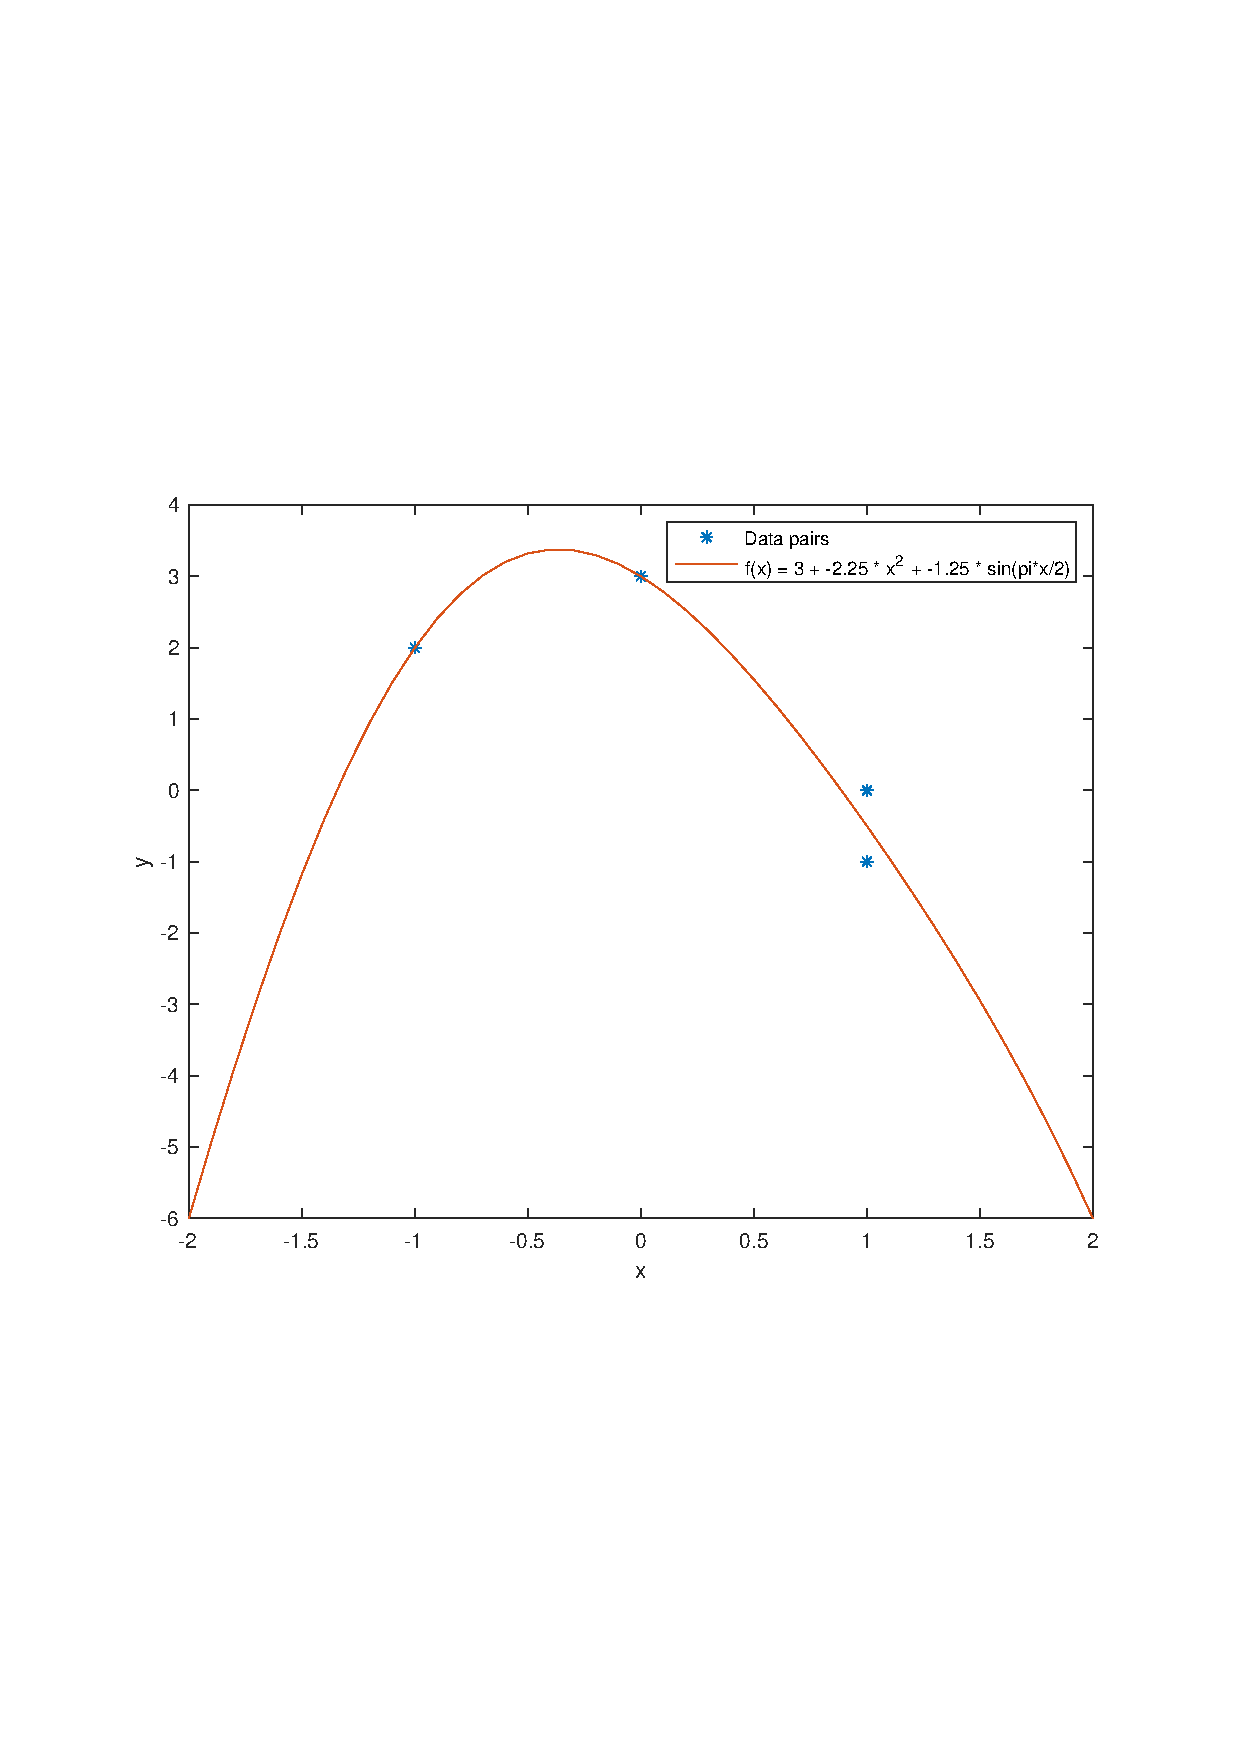
\includegraphics[]{images/Problem_2_a_plot.pdf}
\end{figure}
